\chapter{Results From Flight Data}\label{ch:FlightResult}

This chapter discusses the results of applying the proposed
CC-EKF-SLAM algorithm on realistic aerial video and navigation data.
Firstly, a video of 400 frames was processed by the CC-EKF-SLAM
algorithm. The convergence, consistency, and accuracy of the result
were analyzed against ground truth, and described in Section
\ref{sec:flight-converge}-\ref{sec:flight-accuracy}. While analyzing
pure natural scene video, it was difficult to judge the correctness of
the correspondence between the estimated landmarks and the ground
truth due to the lack of distinguishable visual features. Therefore,
an another video where landmarks can be manually and distinctively
matched was processed, and the result is summarized in Section
\ref{sec:flight-manual}.

The flight test result proved the feasibility of the CC-EKF-SLAM in
mapping object at over 1000 meters distance. When equipped with a high
resolution high dynamic range camera, the system would be able to
produce high resolution model of the surrounding environment, and
detect static obstacles such as tall trees, steep hills, electrical
power line towers, etc.

\section{Convergence Analysis}\label{sec:flight-converge}
When a landmark was added to the filter, the landmark initialization
point was initialized to the zero which is the origin of the camera
reference frame. $\varphi$ and $\theta$ were calculated directly from
the landmark position on the image plane. Therefore they had relatively
high accuracy, and should stay relatively constant. The only parameter
that experienced a converging process was the inverse depth $\rho$,
which was initialized to 0.01 for all landmarks.

\subsection{Convergence of Inverse Depth}
Figure \ref{fltfig:1} shows the $1/\rho$ plot for the entire 400
frames. Landmarks added at the 1$^{st}$ frame are drawn in grey lines.
Landmarks added at later frames are drawn in blue lines. Landmarks
that drifted away are drawn in red line. The Landmark IDs are also
shown on the right side of the plot for these drifting landmarks. The depth
estimates go through rapid changes for several frames after
initialization. Within approximately 20 frames, most inverse depth
estimates have settled to stable values. Sharp spikes in the middle of
the tracking are due to the addition of new landmarks into the filter.
The estimated landmark distances ranged from 400 meters to about 1200
meters, confirming the algorithm's capability for estimating landmarks
at great distance. On the other hand, some landmarks take a long time
to settle, while some others never settle and drift away as tracking
continues, such as landmarks 32, 13, and 53.
% An outlier filter should be in place to get rid of the poor features
% (future work).

\begin{figure}[h]
\centering
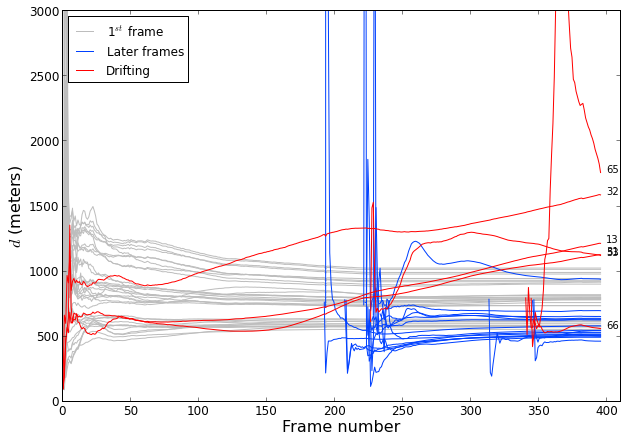
\includegraphics[width=12cm, keepaspectratio=true]{./Figures/fltfig/cut1/Figure131.png}
\caption{Inverse depth convergence}
\label{fltfig:1}
\end{figure}

The non-converging landmarks are those located at the edge of a hill
where objects with a big difference in distance meet in the image. As
an example, the visual pattern of landmark 13 at frame 50, 100, 150,
200, 250, 300, 350 and 398 are shown in Figure \ref{fltfig:1_1}. It
shows that the initial visual pattern for landmark 13 is detected at
the immediate hill top. As the frame number advances, the camera view
becomes different. The pattern comparison in the pyramid LK tracking
algorithm normally allows for a small error at each iteration to
tolerate the slight view change of the camera. This error accumulates
slowly and eventually causes the tracked target to become a pattern
located at a different location, which explains the slow drift in the
depth estimate. To increase the reliability of the estimates, it is
necessary to add a procedure into the algorithm that detect and handle
such behavior.

\begin{figure}[h]
\centering
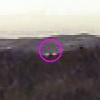
\includegraphics[width=3cm,
keepaspectratio=true]{./Figures/fltfig/cut1/features/uav2_cut1_050_fID13.jpg}
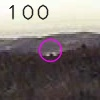
\includegraphics[width=3cm,
keepaspectratio=true]{./Figures/fltfig/cut1/features/uav2_cut1_100_fID13.jpg}
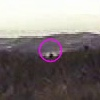
\includegraphics[width=3cm,
keepaspectratio=true]{./Figures/fltfig/cut1/features/uav2_cut1_150_fID13.jpg}
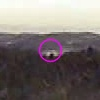
\includegraphics[width=3cm,
keepaspectratio=true]{./Figures/fltfig/cut1/features/uav2_cut1_200_fID13.jpg}
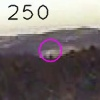
\includegraphics[width=3cm,
keepaspectratio=true]{./Figures/fltfig/cut1/features/uav2_cut1_250_fID13.jpg}
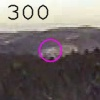
\includegraphics[width=3cm,
keepaspectratio=true]{./Figures/fltfig/cut1/features/uav2_cut1_300_fID13.jpg}
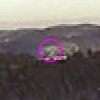
\includegraphics[width=3cm,
keepaspectratio=true]{./Figures/fltfig/cut1/features/uav2_cut1_350_fID13.jpg}
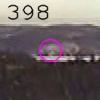
\includegraphics[width=3cm,
keepaspectratio=true]{./Figures/fltfig/cut1/features/uav2_cut1_398_fID13.jpg}
\caption{Landmark 13 at frame 50, 100, 150, 200, 250, 300, 350, and 398}
\label{fltfig:1_1}
\end{figure}

\subsection{Convergence of the Other Landmark Parameters}
When landmarks were initialized, the initialization coordinates $[x_i,
y_i, z_i]$, and the elevation-azimuth angle pair $[\varphi, \theta]$
do not go through a slow converging stage. Ideally, these parameters
should stay at a relatively fixed value. As these parameters were used
with the inverse depth to calculate landmark coordinates on the image
plane and received a corrections at every iteration, their values were
affected by the inverse depth, and varied at each iteration. The plots
in Figure \ref{fltfig:2} show these parameters and their errors over
the entire length of processed frames. The colors of the lines
represents the landmark IDs, which were assigned sequentially when
landmarks were initialized. The ground truth values of these
parameters were extracted using the method described in Section
\ref{sec:flight-accuracy}.

The first column of the plots shows landmark initialization
coordinates. The second column shows the errors of landmark
initialization coordinates. All landmarks initialized at time 0 had
stable values on initialization coordinates, with little variation and
little error. Landmarks that were added at later frames showed drift
from their initial values, as well as offset. The drift is a direct
result of the filter correction process. When a new landmark was added
to the filter, it had not established correlation with all the other
landmarks and the world frame parameters, which caused its correction
on the initialization point to be slightly different than all the
existing landmarks and the world frame position. As a future
improvement, it is reasonable for the newly added landmark to inherit
the cross-correlation on the initialization coordinates from a
landmark close to it. The biggest errors on landmark initialization
coordinates for landmarks added at later frames come from the offset
errors. The offset errors are very significant on the Y axis. Since
the landmark initialization coordinates are highly correlated to the
SUAS location estimates, the offset errors are direct results of the
errors in SUAS localization estimates. A more detail analysis is given
in Section \ref{sec:landmarkMotion}

The third and fourth columns of Figure \ref{fltfig:2} show elevation
angle $\varphi$, azimuth angle $\theta$, and their errors. For all
landmarks, whether initialized at the first image frame or later frames,
these angle estimates all diverged slightly from the initial values.
There were two factors that contributed to the variation of $\varphi$
and $\theta$. Firstly, the initial depths of the landmarks were
unknown. To compensate for the incorrect depth, the filter must adjust
$\varphi$ and $\theta$ estimates slightly so that the predicted
measurements agree with the actual measurements. Secondly, big
variations in the estimates were seen at around frame 200 when a lot
of new landmarks were added to the filter. This observation suggests
that an addition of new landmark has negative impact on the accuracy of
estimates. Therefore additions of new landmarks should not be allowed
to happen too frequently in order to limit their effects. For
landmarks initialized at later frames, offset errors at initialization
were much more significant, and were accounted for the majority of the
mapping errors seen in those landmarks. Further discussion on the offset
errors for these landmarks are presented in Section
\ref{sec:landmarkMotion}
% doesn't make sense. By definition, X rotation should have bigger
% impact on varphi, Z rotation has bigger impact on theta

\begin{figure}[h]
\centering
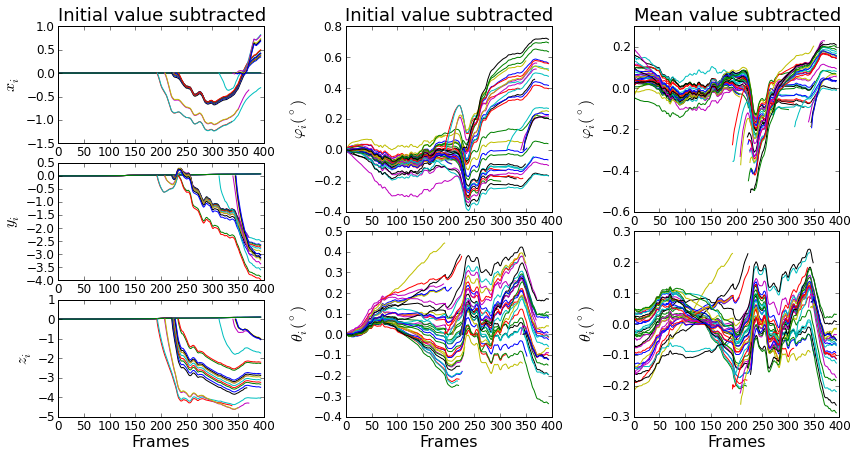
\includegraphics[width=15cm, keepaspectratio=true]
{./Figures/fltfig/cut1/Figure20.png}
\caption{Convergence and errors of all other landmark parameters
  besides inverse depth}
\label{fltfig:2}
\end{figure}
% THIS WAS THE OLD TEXT, MAY NOT BE TRUE. On the other hand, features
% mapping is not affected too much by the error in localization.
% Because their parameters are transformed in each iteration to the
% new camera frame using the estimated SUAS motion which carries the
% error. As long as their parameters are updated together with the
% estimated motion on that iteration, and transformed back to the
% world frame using the same estimated motion, the final result of
% features location in world frame is unaffected by the error in the
% SUAS localization. However, for feature removed from the filter,
% their parameters are no longer updated, therefore revealing the
% error in SUAS localization.
\FloatBarrier

\section{Consistency Analysis}\label{sec:flight-consistency}
Research on EKF SLAM properties indicated that 
\begin{enumerate}
  \item An EKF system becomes inconsistent when the variance of a state
  vector element becomes too small and forbids an effective correction,
  \item Uncertainty of the world frame should increase as the
  camera frame moves away from the world frame origin.
\end{enumerate}

To examine the consistency of the CC-EKF-SLAM algorithm, the variance
of world frame parameters and camera motions are plotted in Figure
\ref{fltfig:120}, and the variance of landmark parameters are plotted
in Figure \ref{fltfig:3}. The variance of world frame position
increases with iterations at the beginning. After frame 100,
$\sigma^2_{O_Y}$ and $\sigma^2_{O_Z}$ converge to a relatively stable
value. This is likely due to the small and slow variation on the Y and
Z translation of the SUAS. On the other hand, camera rotation and
world frame orientation variance have a similar pattern and amplitude.
The X component of world frame orientation decreases with iterations,
while Y and Z components fluctuate around a fixed value and remain
below 1.5e-5$^\circ$. Landmark parameters $\varphi$ and $\theta$ also
have very small variance since they are affected by the variance of
camera rotation. In the CC-EKF-SLAM algorithm, although the world
frame orientation variance remains fixed at the prediction step,
camera rotation variances have 0.1$^\circ$ of noise added (as indicated
by the GS-111m specification \cite{_athena_????}). An investigation
into the algorithm shows that the EKF correction step reduces the noise of
camera rotation significantly and results in a variance estimate much
lower than the specification.

% does increasing measurement variance increases parameter variance?
% answer: NO 

\begin{figure}[h]
\centering
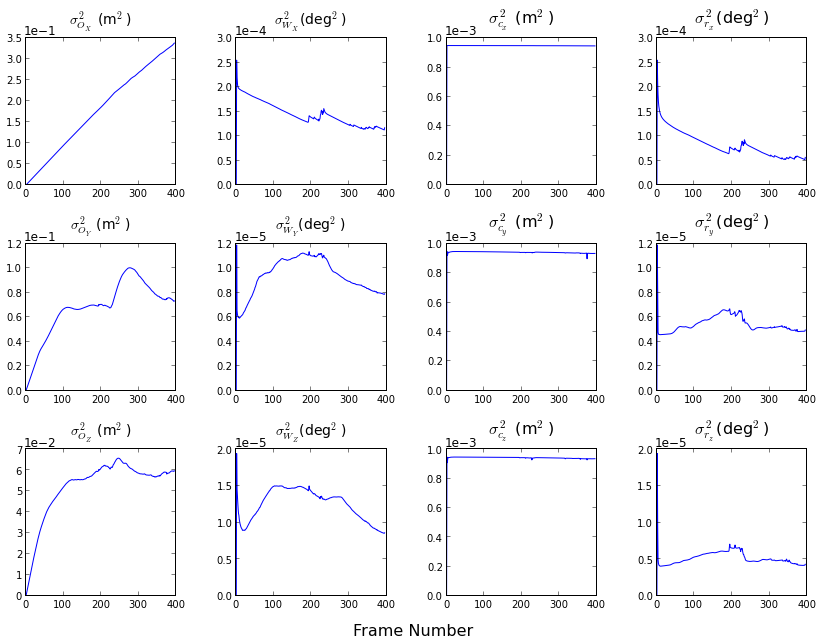
\includegraphics[width=14cm, keepaspectratio=true]
{./Figures/fltfig/cut1/Figure120.png}
\caption{Variance of world frame parameters and camera motion}
\label{fltfig:120}
\end{figure}


\begin{figure}[h]
\centering
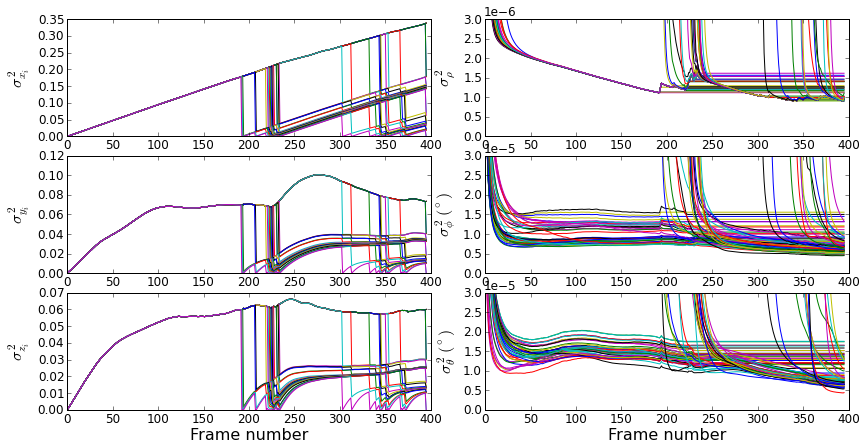
\includegraphics[width=14cm, keepaspectratio=true]
{./Figures/fltfig/cut1/Figure40.png}
\caption{Variance of landmark parameters}
\label{fltfig:3}
\end{figure}
\FloatBarrier

% consider deleting first and second point in the paragraph. Only the
% third point leads to explaination of error.
To see the effect of small variance on the correction process of
CC-EKF-SLAM, correction amounts applied to the predicted state vector
are plotted in Figure \ref{fltfig:4}. It can be observed that in
general the correction amounts agree with the variance in that a
bigger variance results in more correction, except for the world frame
position and camera translation on Y and Z axes. These parameters
receive more correction as tracking progresses despite their variance
being stabilized or even decreasing. Secondly, there is a strong
correlation between the landmark initialization positions, the world
frame positions, and camera translation estimates. World frame
positions and landmark initialization positions are inversely
correlated to the camera translations on Y and Z axes. Thirdly, the
camera parameter corrections show an obvious trend on Y and Z
translation. The correction amounts on camera translation on Y and Z axes
are increasing with time. Due to these relationships, the main
contributor for drift in SUAS position and offset in landmark mapping
should be the camera translation correction on Y and Z axes. On the
other hand, the big correction on these parameters could be caused by
the small variance in the camera rotation. If not enough correction
can be made into the camera rotation and $\varphi$ and $\theta$
angles, the algorithm must compensate that by making more adjustment
in the camera translation on the Y and Z axes. This issue requires
further investigation, and will be analyzed in future work.

\begin{figure}[h]
\centering
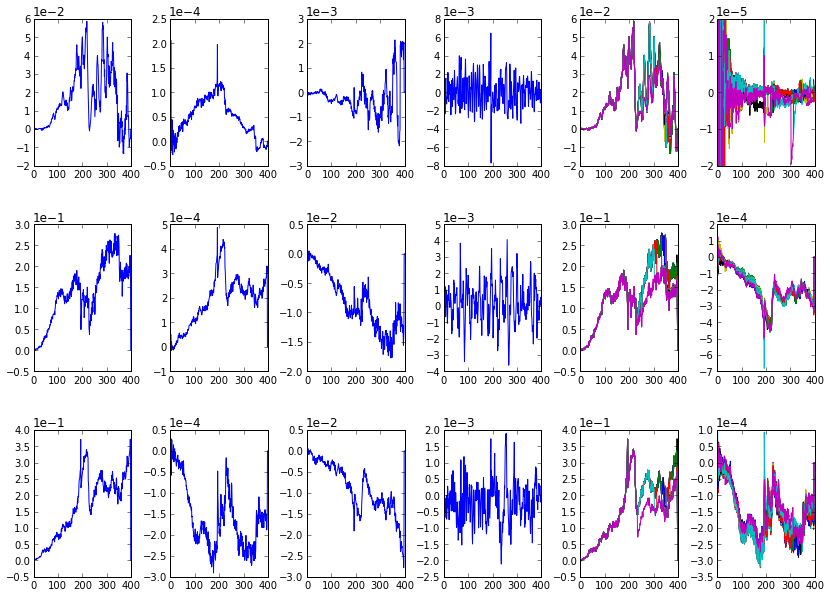
\includegraphics[width=15cm, keepaspectratio=true]
{./Figures/fltfig/cut1/Figure112.png}
\caption{Plot of corrections applied to state vector}
\label{fltfig:4}
\end{figure}
\FloatBarrier

\section{Accuracy Analysis}\label{sec:flight-accuracy}
\subsection{SUAS Localization}

Ground truth for SUAS positions and orientations came from the GPS,
and magnetometer. The GPS positioning can generally achieve 7.8 meters
in accuracy \cite{_gps_????}. For orientation, accuracy on the GS-111m
datasheet specifies $0.1^{\circ}$ for roll and pitch, and
$0.5^{\circ}$ for heading. Figure \ref{fltfig:6} shows the estimated
SUAS position and orientation, the ground truth, and the error. From the
comparison, X position error reaches a maximum of 4.8 meters, while
error in Y and Z are bigger, reaching 60 meters and 28 meters
respectively. The position on the Y axis is clearly diverging from the
ground truth by the end of 400 frames. For orientation, the estimated
value agreed with the ground truth pattern, with maximum error within
0.02 rad or $1.15^{\circ}$. There is no clear sign of divergence
within the 400 frames processed. Another characteristic that can be
observed is the correlation between the position errors and the
aircraft orientation. Error on the Y position is correlated to the
orientation on the Z axis; error on the Z position is correlated to the
orientation change on Y axis. Clearly, aircraft rotational motion
plays a crucial part on the accuracy of the estimates.

\begin{figure}[h]
\centering
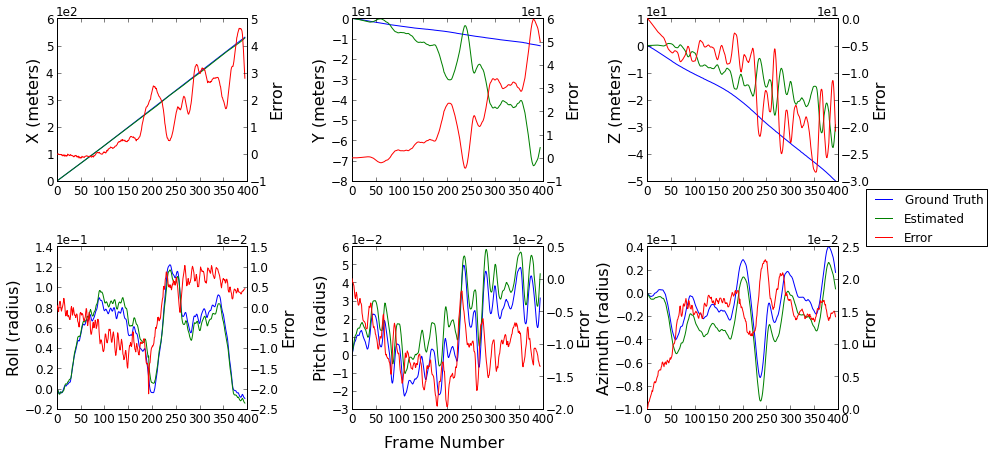
\includegraphics[width=15.5cm, keepaspectratio=true]
{./Figures/fltfig/cut1/Figure30.png}
\caption{SUAS poses compared to ground truth for the natural scene video}
\label{fltfig:6}
\end{figure}
\FloatBarrier

\subsection{Landmarks Mapping}\label{sec:accuracy_features}

The ground truth data came from the digital elevation map (DEM) which
was downloaded from the CGIAR-CSI website \cite{_cgiar-csi_????}. The
DEM has approximately 90 meters resolution, and the reported vertical
error is less than 16 meters. The map was interpolated when being
compared to the estimated landmark position. 

Establishing a data correspondence between the DEM and the estimated
landmarks is non-trivial for a natural scene which lacks
distinguishable visual features such as building corners or other
man-made objects. As shown in the converging plots Figure
\ref{fltfig:2}, landmark parameters do experience drift in flight.
Hence, the best time for achieving data correspondence with the DEM is
when landmarks are first initialized. At the time of initialization,
landmark initialization positions $[x_i, y_i, z_i]$ were zeros.
$[\varphi, \theta]$ were calculated from landmark coordinates in the
image, and did not carry any error contributed by the unknown $\rho$
or the pyramid LK algorithm. Therefore, the following procedure was
used to find the corresponding ground truth location for every
estimated landmark.

\begin{enumerate}
  \item Identify the frame number at which a landmark is initialized.
  Record the ground truth position of the SUAS at that frame.
  \item Create a reference frame aligned with the UTM frame on DEM
  using the ground truth SUAS position.
  \item Convert the landmark parameters $\theta$ and $\varphi$
  angles at initialization from the camera frame to the reference frame created in step 2. 
  \item Create a vertical plane using $\theta$ to slice the DEM to
  form a 1D elevation plot. An example is shown by the blue line in Figure
  \ref{fltfig:7}.
  \item Create a line using $\varphi$ to intersect the 1D elevation plot
  (Figure \ref{fltfig:7} green line). 
  \item The $1^{st}$ intersection is used as the ground truth landmark
  location.
\end{enumerate}

\begin{figure}[h]
\centering
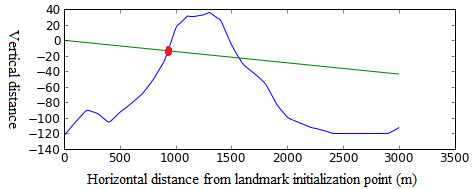
\includegraphics[width=10cm, keepaspectratio=true]
{./Figures/fltfig/find_groundtruth.png}
\caption{Finding ground truth landmark position on DEM}
\label{fltfig:7}
\end{figure}

The convergence of landmark position errors is plotted in Figure
\ref{fltfig:8}. Landmarks added at the 1$^{st}$ frame are drawn in
grey lines. Landmarks added at later frames are drawn in blue lines.
Landmarks that drifted away are drawn in red lines. The errors on the
X component (along which axis the SUAS was traveling) converge to zero
in general, with the amount ranging from 2.8 meters to 120 meters. The
errors on the Y component show clear offsets for landmarks not
initialized at the first frame. This behavior is similar to what is
seen in the error analysis in Section \ref{sec:landmarkMotion} where
offset in landmark position estimates are caused by drift in UAV
localization estimation. Offsets on the Z component are much less
obvious.

\begin{figure}[h]
\centering
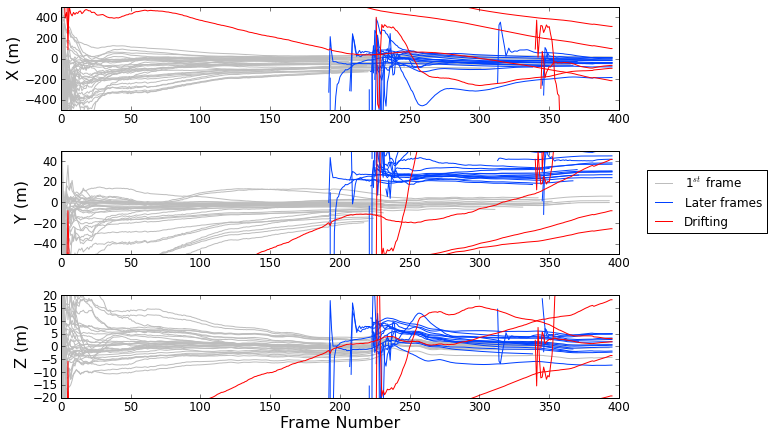
\includegraphics[width=14cm, keepaspectratio=true]
{./Figures/fltfig/cut1/Figure500.png}
\caption{Landmark position errors convergence in world frame}
\label{fltfig:8}
\end{figure}

Landmark IDs were assigned to landmarks sequentially when landmarks
were initialized into the filter. Plotting the estimated and ground
truth landmark positions against landmark IDs revealed more detail on
the errors. Figure \ref{fltfig:9} shows the estimated and ground truth
landmark positions on the left, and the errors on the right. On X and
Z axes, the biggest error occurs on landmark 65 which was initialized
fairly late in the sequence, and may not have converged properly.
Other landmarks that carry big errors, such as landmarks 13, 31, and
32, are all located on the hill top in the image of Figure
\ref{fltfig:line_features}. The visual tracking problem discussed
earlier applies to all these line features. Hence, accuracy of
distance estimates on these landmarks were affected. On the Y axis,
the plots show that landmarks with IDs higher than 40 have offset
errors. All landmarks with IDs higher than 40 were initialized after
frame 180, at which point the SUAS had travelled away from the world
frame origin for at least 200 meters. In general, the average error
increases as landmark ID gets bigger, which indicates that the further
the landmark initialization point is from the world frame origin, the
bigger the offset error becomes. A more detail analysis was done to
find the source of these offset errors, and the results are presented
in Chapter \ref{ch:simulation}. The statistics of landmark position
errors are summarized in Table \ref{tab:lm_err_stats_nat}.

\begin{figure}[h]
\centering
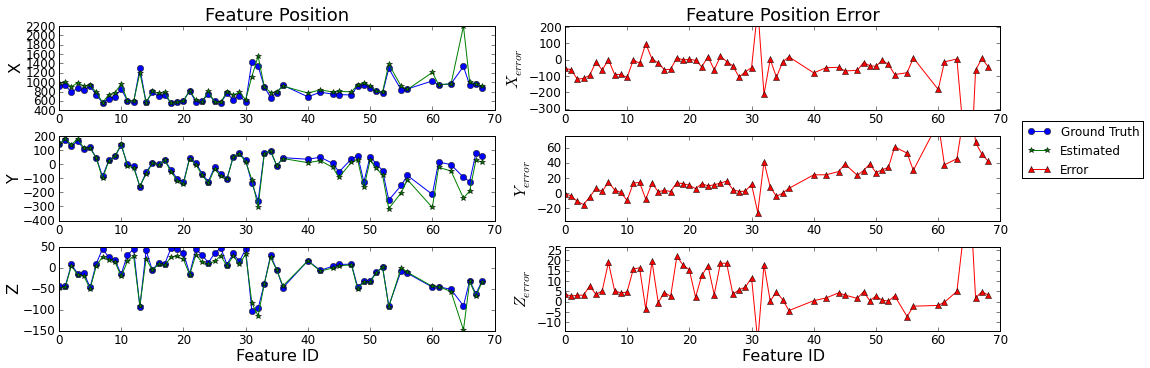
\includegraphics[width=16cm, keepaspectratio=true]
{./Figures/fltfig/cut1/Figure60.png}
\caption{Landmark positions and errors plotted against initialization
  sequence for the natural scene video}
\label{fltfig:9}
\end{figure}
\FloatBarrier
\begin{table}[h]
\caption{Landmark mapping error statistics for natural scene}
\label{tab:lm_err_stats_nat}
\centering
\begin{tabular}{|c|c|c|}
\hline
          & Mean       & Standard Deviation \\ \hline
$X_{error}$ & -56.21 meters    & 136.23 meters            \\ \hline
$Y_{error}$ & 13.75 meters     & 31.01 meters             \\ \hline
$Z_{error}$ & 1.34 meters      & 9.09 meters              \\ \hline
\end{tabular}
\end{table}      

\begin{figure}[h]
\centering
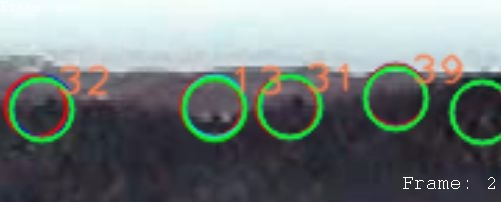
\includegraphics[width=7cm, keepaspectratio=true]
{./Figures/fltfig/landmark_13_31_32.jpg}
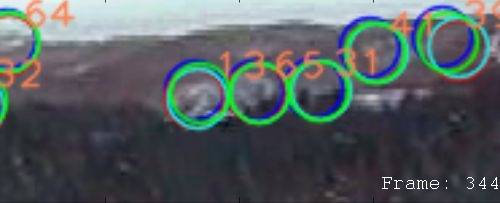
\includegraphics[width=7cm, keepaspectratio=true]
{./Figures/fltfig/landmark_13_65_32.jpg}
\caption{Visual appearance of landmark 13, 31, 32, and 65}
\label{fltfig:line_features}
\end{figure}

Using the estimated landmark positions, a terrain map can be
generated. Figure \ref{fltfig:10} shows the resulting terrain map on
the left with landmarks marked by circle markers. On the right, the
ground truth DEM is also shown for comparison. The estimated terrain
map agrees with the DEM at location where sufficient amount of
landmarks can be established, such as the front and right side of the
map.

\begin{figure}[h]
\centering
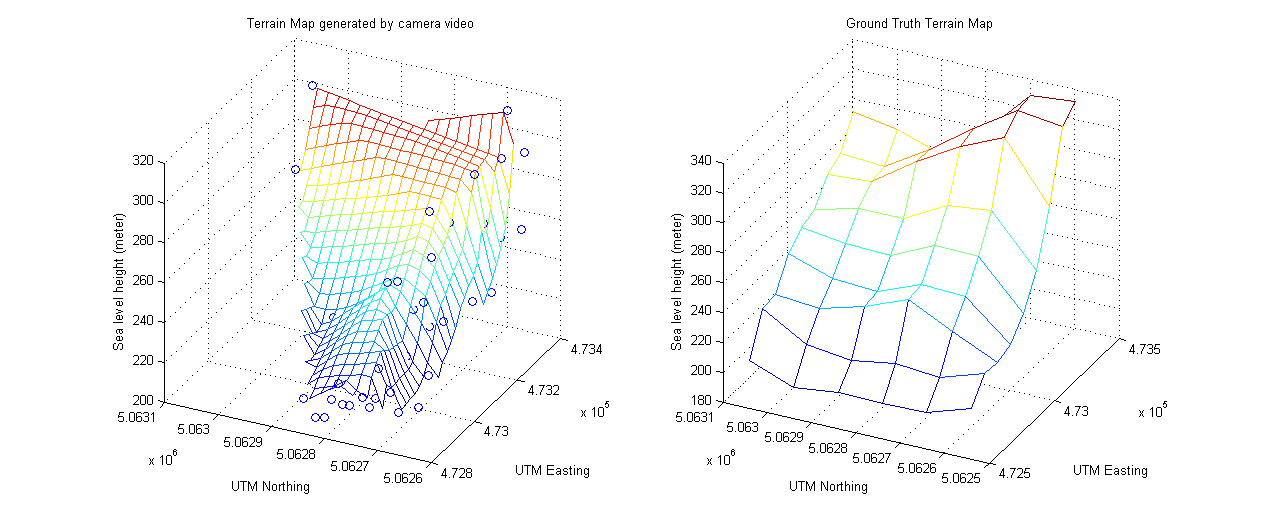
\includegraphics[width=14cm, keepaspectratio=true]
{./Figures/fltfig/cut1/terrain/terrain_map_cmp.png}
\caption{Terrain map comparison. Left: terrain map generated from
  estimated landmarks. Right: the digital elevation map (DEM). }
\label{fltfig:10}
\end{figure}
\FloatBarrier

\section{Accuracy Verification through Manually Corresponded Landmarks}
\label{sec:flight-manual}
Due to the difficulty in corresponding estimated landmarks to the DEM,
a second piece of video was processed with man-made
structures in the scene so that landmark correspondence can be made
manually. Ground truth on landmark coordinates were taken from Google
Earth. Since Google Earth provides very rough elevation data,
ground truth on landmark elevations were taken from the GPS measurements of the
helicopter after it had landed at the airport. Figure \ref{fltfig:11}
shows a zoomed-in view of the landmarks extracted by the CC-EKF-SLAM.
All landmarks are located at the bottom left corner of the image.
Figure \ref{fltfig:12} shows the common landmarks found manually on
the satellite image on Google Earth \cite{_google_????}.

\begin{figure}[h]
\centering
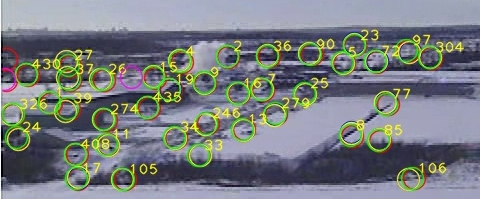
\includegraphics[width=10cm, keepaspectratio=true]
{./Figures/fltfig/airport/frame398_landmarks.jpg}
\caption{Landmarks extracted by algorithm from the airport landing video }
\label{fltfig:11}
\end{figure}

\begin{figure}[h]
\centering
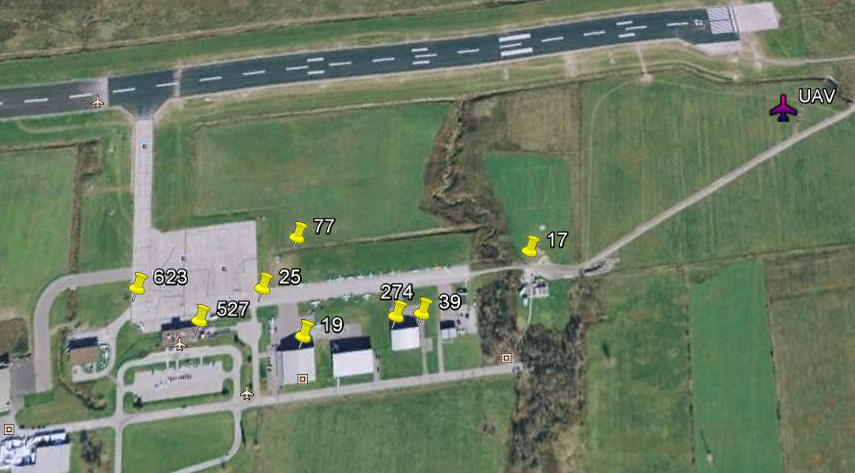
\includegraphics[width=13cm, keepaspectratio=true]
{./Figures/fltfig/airport/uav_and_identified_landmark.png}
\caption{Common landmarks manually identified on Google Earth }
\label{fltfig:12}
\end{figure}
\FloatBarrier 

The estimated SUAS poses are compared to the GPS
and IMU recordings in Figure \ref{fltfig:13}. Similar to the natural
scene video, SUAS position estimates are more accurate on X and Z,
and experience more drift on the Y axis. The drift becomes significant
when the frame number exceeds 200. The correlation between the position errors
and the rotational motions of the aircraft can also be found in this
plot.

\begin{figure}[h]
\centering
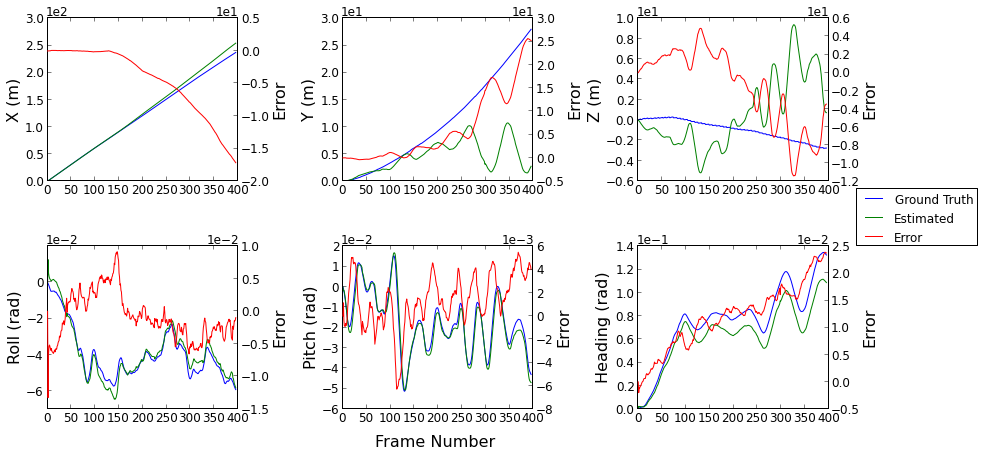
\includegraphics[width=17cm, keepaspectratio=true]
{./Figures/fltfig/airport/Figure10.png}
\caption{SUAS poses compared to ground truth for the airport landing video}
\label{fltfig:13}
\end{figure}
\FloatBarrier

Figure \ref{fltfig:15} shows the landmark positions compared to ground
truth. This plot shows a clear offset error between the ground truth
and the estimated. The error statistics are given in Table
\ref{tab:lm_err_stats_airport}. Compared to the landmark error
statistic from natural scene video, these errors have bigger mean, but
much smaller standard deviation. This suggests that the landmarks
might be affected by specific error source. Since the offset errors
exist on all landmarks regardless of their ID value, and all landmarks
are located at the bottom left corner of the FOV, it is likely that
lens distortion is the main contributor for these errors. On the other
hand, the error from airport landing video are within $3\sigma$ of the
error statistics established in the natural scene video. The
statistics comparison confirms that the accuracy analysis result from
both videos agrees in general, and that the ground truth to estimated
landmark correspondence method used in natural scene is valid.


\begin{figure}[h]
\centering
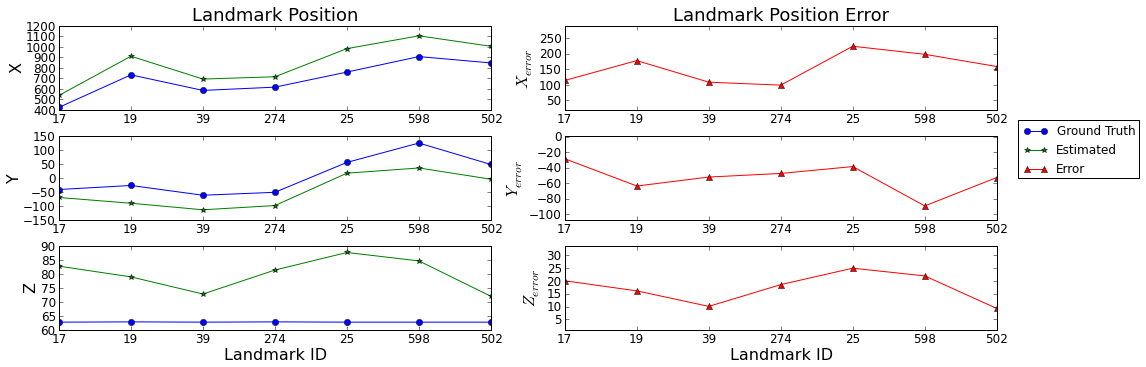
\includegraphics[width=17cm, keepaspectratio=true]
{./Figures/fltfig/airport/Figure20.png}
\caption{Landmark positions and errors for the airport landing video}
\label{fltfig:15}
\end{figure}

\begin{table}[h]
\caption{Landmark mapping error statistics for airport landing scene}
\label{tab:lm_err_stats_airport}
\centering
\begin{tabular}{|c|c|c|}
\hline
          & Mean       & Standard Deviation \\ \hline
$X_{error}$ & 154.33 meters    & 44.86 meters            \\ \hline
$Y_{error}$ & -53.15 meters     & 17.98 meters             \\ \hline
$Z_{error}$ & 17.27 meters      & 5.44 meters              \\ \hline
\end{tabular}
\end{table} 



%%% Local Variables:
%%% mode: latex
%%% TeX-master: "thesis"
%%% End:
